\chapter{Paper III:\@
  Overreact,
  an in silico lab:
  \linebreak
  automative quantum chemical microkinetic simulations
  for complex chemical reactions
 }%
\label{ch:paper3}

\begin{citacao}
	\fullcite{Schneider_2022}
\end{citacao}

In order to overcome the challenges of this century,
such as producing fuels and chemicals from biomass and greenhouse gases,
and developing greener synthetic protocols,
it is necessary to improve the understanding of reaction mechanisms.
One way of accomplishing this is through the use of computational modeling tools and methodologies,
which have become more efficient and accurate due to the growth of computing resources and methodological developments.
However,
these calculations must take into account as much of the relevant physics of the problem as possible,
such as pre-equilibration and concentration,
dispersion corrections,
solvation,
molecular symmetry,
proper treatment of Gibbs energy contributions,
standard state corrections,
quantum tunneling,
and others.

First-principle calculations have been used to calculate binding free energies
and reaction rate constants that are close to what is observed in experiments.
It is thus viable to use calculations from computational chemistry to determine parameters of reactions,
then simulate a microkinetic model for the process.
A clear advantage of this approach is that it is possible to take the concentrations of the reactants into account.
Microkinetic models can be used to analyze and test hypotheses in catalysis and chemical kinetics.
This makes it possible to use first-principles microkinetic simulations to understand complex reactions over time.
However,
there is currently no general solution for first-principles microkinetic modeling
that can do all of the necessary calculations and generate an equation system automatically.

This work introduces a novel Python package,
named \overreact{}.
It is a user-friendly,
open-source program that can be used
to automatically perform microkinetic modelling of complex chemical reactions in solution or gas-phase
using data from first-principles quantum chemical calculations.
All it requires is a description of the hypothesized reactions,
the corresponding computational chemistry output files,
initial concentrations,
and reaction conditions such as temperature.
It is compatible with 14 widely available computational chemistry packages
(by making use of the~\cclib{}~library~\cite{O_boyle_2008})
and can be used to simulate reactions in both neat and buffered conditions.
\overreact{}~supports a variety of quantum chemistry methods,
from density functional theory to wavefunction methods,
as well as composite models (e.g.,
DLPNO-CCSD(T)/cc-pVTZ//PBE0-D4/def2-TZVP),
as long as the data is parseable by~\cclib{}~\cite{O_boyle_2008}.
It also allows the user to correct systematic errors in first-principle absolute Gibbs energy errors
by the use of a single tunable parameter.
This is important for bimolecular reactions,
and a correction can be easily obtained by fitting systematic deviations
in first-principles reaction schemes by using available experimental data,
for instance.

The software is useful to inspect steady-state conditions,
search for predominant species under catalytic conditions,
computationally estimate the overall turn-over frequency and understand selectivity of a catalyst towards particular products.
It allows rapid rational design and investigation in those areas where understanding how reactions work is important,
and provides insight into concentration dependencies and comparison with experiment,
since it performs microkinetic simulations
and thus produces kinetic profiles.
Kinetic models can be progressively constructed,
with given pathways,
thereby increasing human efficiency.

Some reaction examples were performed in the work,
all using the default settings.
For instance,
the estimated autoisomerization rate of ethane from staggered to eclipsed
and back to staggered was found to agree with experimental value.
The reaction rate constant for the umbrella inversion of ammonia was estimated to agree
with the experimental value of $4 \times 10^{10}$~s$^{-1}$.

In the context of gas-phase reactions,
we modelled the degradation of methane degradation by chlorine radicals,
an important atmospheric chemistry reaction.
\linebreak
\overreact{}~provided reaction rate constants consistent with both
experimental
values
($1.0 \times 10^{-13}$~cm$^3$~molecule$^{-1}$~s$^{-1}$~\cite{Burkholder_2020})~and computational calculations
by~\citeauthor{Tanaka_1996}~\cite{Tanaka_1996}.

In the context of solvated-phase,
M06--2X-D3(0)/6--311++G(d,p)/SMD was used to estimate the rate constant for \ce{NH3_{(w)} + OH._{(w)} -> NH2._{(w)} + H2O_{(w)}}.
at high~pH,
with values agreeing with experimental results.
We also reproduced the results by~\citeauthor{P_rez_Soto_2020},
who applied computer-aided analysis
to study an imine formation reaction,
taking into consideration the catalytic effect of small amounts of water in the milieu,
either as contamination from residuals in the solvent
or due to its formation as a by-product.
Such systems can be complex and require microkinetics or other techniques to properly explain them,
as direct consideration of concentrations through time is required.
In total,
the system simulates 25 simultaneous reactions and 17 species.

We investigated the mechanism of intramolecular amide hydrolysis,
with three proposed mechanisms replicated.
Since it is known that the reaction is strongly dependent on~pH,
we used the experimentally derived pK$_a$ of acetic acid to correct all acid-base equilibria.
From simulations at different~pH~values,
it was also found that the reaction rate is strongly affected by the~pH,
and that it stops happening around~pH~5,
as expected from experimental results.

In fact,
by simulating the system for an hour at a~pH~of~2
and observing the concentrations of different intermediates over time,
we could reproduce the experimental fact that
the reaction only takes place in acidic environments.
Furthermore,
it was observed that the reaction rate increases significantly when
a single water molecule actively participates as a proton shuttle,
as proton transfer in a four-membered ring transition state is rate-determining.

To conclude,
we discussed a software for obtaining reaction kinetic profiles from first-principle calculations.
The package is automated and makes it easy for computational discoveries in the elucidation of reaction mechanisms
to be compared with experimentally obtained results,
which is crucial for studying chemical reactions.
The open-source package presented in this article is available to explore and analyze reaction mechanisms.
The software is suitable for predicting catalysts performance at scale,
which is crucial for the emergent need for rapid and precise chemical modelling.

\section{Paper}

The \overreact{}~software was developed at the Department of Chemistry at the Federal University of Santa Catarina (UFSC).
It can be regarded as a second iteration on a previous attempt to build a chemical kinetics simulator~\cite{pyrrole2019zenodo}.
The code is released under the permissive MIT open-source license~\cite{MITLicense}.

This research was funded by the Brazilian Council for Scientific and Tecnological Development (CNPq),
grant/award numbers 140485/2017--1 and 311132/2020--0.

The publication can be read in full next.
Reprinted with permission from
\fullcite{Schneider_2022}.
Copyright~\citeyear{Schneider_2022}
John~Wiley~\&~Sons,~Inc.

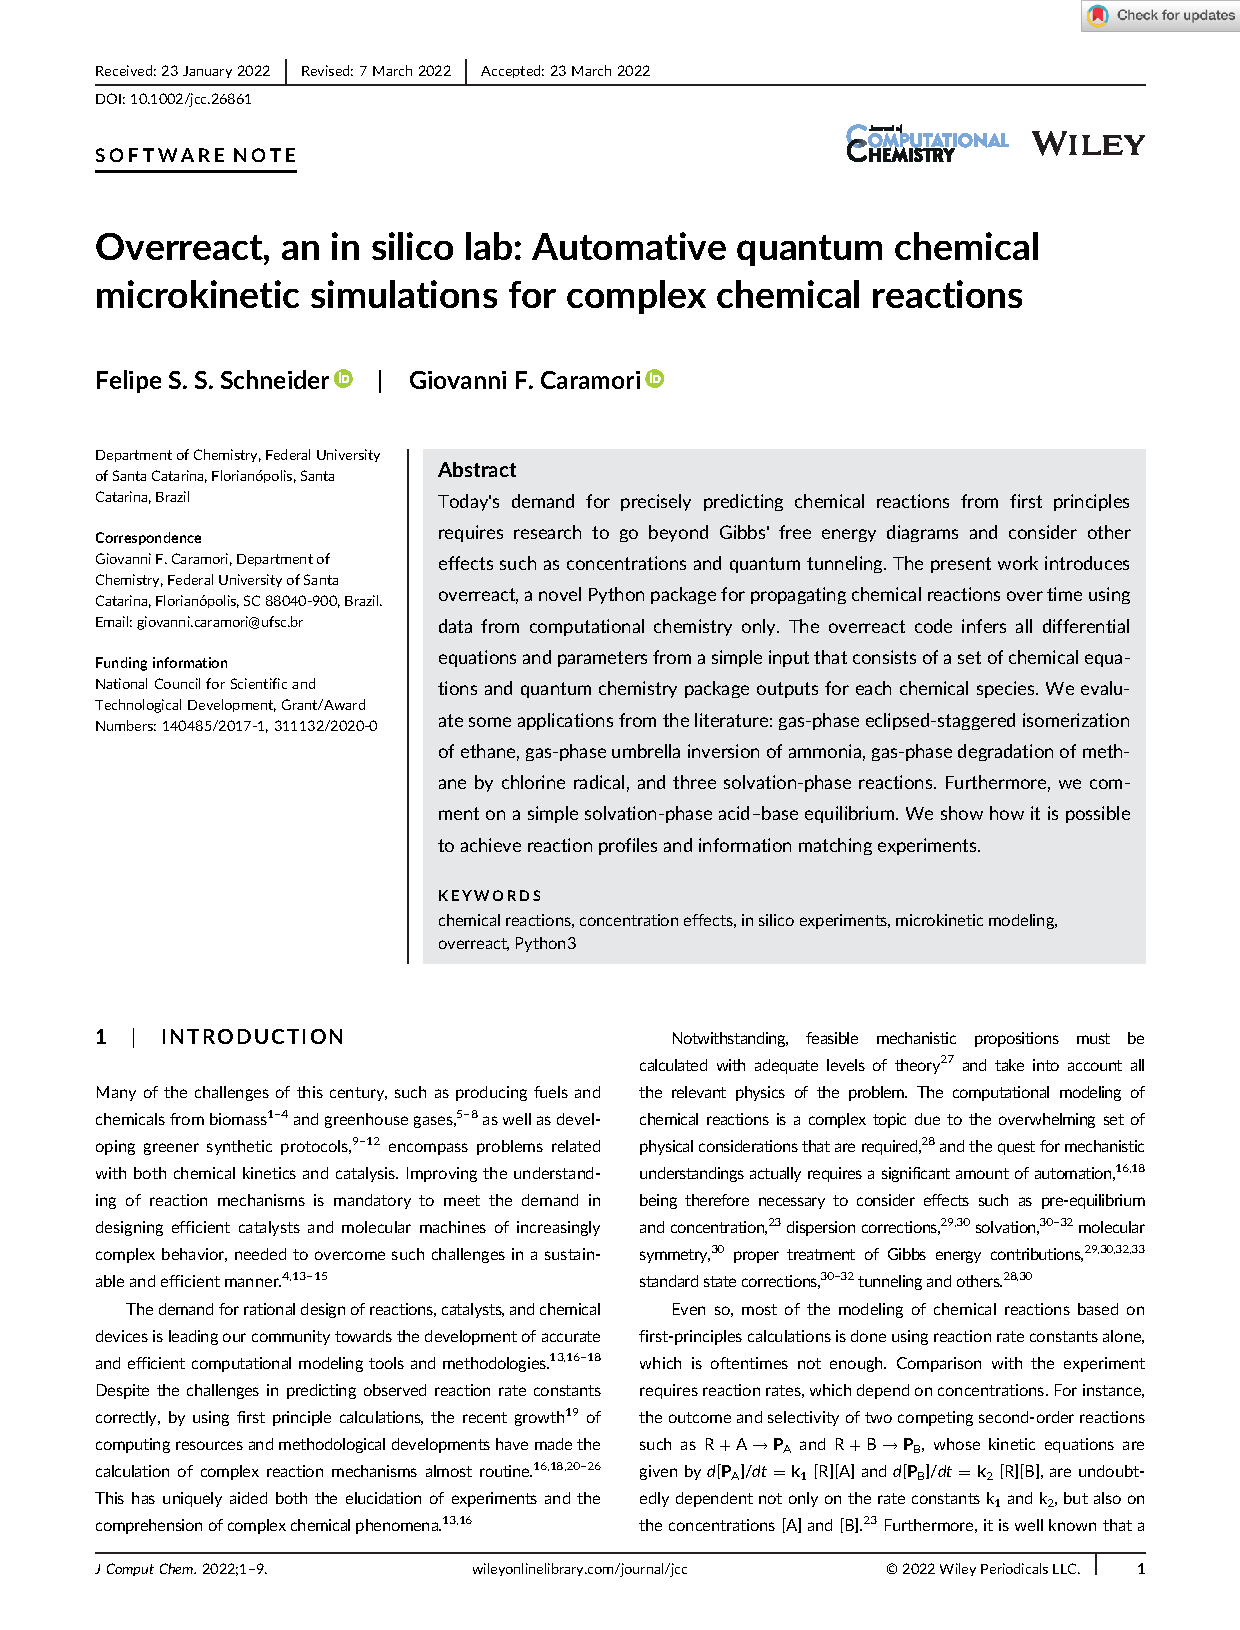
\includepdf[pages=-]{pubs/schneider2022-paper3.pdf}
